\documentclass[12pt]{report}
\usepackage[utf8]{inputenc}
\usepackage[russian]{babel}
%\usepackage[14pt]{extsizes}
\usepackage{listings}
\usepackage{graphicx}
\usepackage{csvsimple}
\usepackage{amsmath,amsfonts,amssymb,amsthm,mathtools} 
\usepackage{pgfplots}
\usepackage{filecontents}
\usepackage{indentfirst}
\usepackage{eucal}
\usepackage{float}
\usepackage{amsmath}
\usepackage{enumitem}
\frenchspacing

\usepackage{indentfirst} % Красная строка


%\usetikzlibrary{datavisualization}
%\usetikzlibrary{datavisualization.formats.functions}

\usepackage{amsmath}


% Для листинга кода:
\lstset{ %
	language=haskell,                 % выбор языка для подсветки (здесь это С)
	basicstyle=\small\sffamily, % размер и начертание шрифта для подсветки кода
	numbers=left,               % где поставить нумерацию строк (слева\справа)
	numberstyle=\tiny,           % размер шрифта для номеров строк
	stepnumber=1,                   % размер шага между двумя номерами строк
	numbersep=5pt,                % как далеко отстоят номера строк от подсвечиваемого кода
	showspaces=false,            % показывать или нет пробелы специальными отступами
	showstringspaces=false,      % показывать или нет пробелы в строках
	showtabs=false,             % показывать или нет табуляцию в строках
	frame=single,              % рисовать рамку вокруг кода
	tabsize=2,                 % размер табуляции по умолчанию равен 2 пробелам
	captionpos=t,              % позиция заголовка вверху [t] или внизу [b] 
	breaklines=true,           % автоматически переносить строки (да\нет)
	breakatwhitespace=false, % переносить строки только если есть пробел
	escapeinside={\#*}{*)}   % если нужно добавить комментарии в коде
}

\linespread{1.5}
\usepackage[left=2cm,right=2cm, top=2cm,bottom=2cm,bindingoffset=0cm]{geometry}
% Для измененных титулов глав:
\usepackage{titlesec, blindtext, color} % подключаем нужные пакеты
\definecolor{gray75}{gray}{0.75} % определяем цвет
\newcommand{\hsp}{\hspace{20pt}} % длина линии в 20pt
% titleformat определяет стиль
\titleformat{\chapter}[hang]{\Huge\bfseries}{\thechapter\hsp\textcolor{gray75}{|}\hsp}{0pt}{\Huge\bfseries}


% plot
\usepackage{pgfplots}
\usepackage{filecontents}
\usetikzlibrary{datavisualization}
\usetikzlibrary{datavisualization.formats.functions}

\begin{document}
	%\def\chaptername{} % убирает "Глава"
	\thispagestyle{empty}
	\begin{titlepage}
		\noindent \begin{minipage}{0.15\textwidth}
			
\includegraphics[width=\linewidth]{b_logo}
		\end{minipage}
		\noindent\begin{minipage}{0.9\textwidth}\centering
			\textbf{Министерство науки и высшего образования Российской Федерации}\\
			\textbf{Федеральное государственное бюджетное образовательное учреждение высшего образования}\\
			\textbf{~~~«Московский государственный технический университет имени Н.Э.~Баумана}\\
			\textbf{(национальный исследовательский университет)»}\\
			\textbf{(МГТУ им. Н.Э.~Баумана)}
		\end{minipage}
		
		\noindent\rule{18cm}{3pt}
		\newline\newline
		\noindent ФАКУЛЬТЕТ $\underline{\text{«Информатика и системы управления»}}$ \newline\newline
		\noindent КАФЕДРА $\underline{\text{«Программное обеспечение ЭВМ и информационные технологии»}}$\newline\newline\newline
		
		
		\begin{center}
			\noindent\begin{minipage}{1.3\textwidth}\centering
				\Large\textbf{  Отчёт по лабораторной работе №6}\newline
				\textbf{по дисциплине "Анализ алгоритмов"}\newline\newline
			\end{minipage}
		\end{center}
		
		\noindent\textbf{Тема} $\underline{\text{Муравьиный алгоритм и метод полного перебора для решения задачи коммивояжёра}}$\newline
		\noindent\textbf{Студент} $\underline{\text{Мицевич М. Д.}}$\newline
		\noindent\textbf{Группа} $\underline{\text{ИУ7-51Б}}$\newline
		\noindent\textbf{Преподаватель} $\underline{\text{Волкова Л.Л}}$\newline\newline\newline\newline
		
		\begin{center}
			\vfill
			Москва~---~\the\year
			~г.
		\end{center}
	\end{titlepage}
	
	
	\tableofcontents
	
\newpage
\chapter*{Введение}
\addcontentsline{toc}{chapter}{Введение}
	
Муравьиный алгоритм -- один из эффективных полиномиальных алгоритмов для нахождения приближённых решений задачи коммивояжёра, а также решения аналогичных задач поиска маршрутов на графах. Суть подхода заключается в анализе и использовании модели поведения муравьёв, ищущих пути от колонии к источнику питания, и представляет собой метаэвристическую оптимизацию.
	
\section*{Цель лабораторной работы}
	
Целью данной лабораторной работы является изучение муравьиного алгоритма и приобретение навыков параметризации методов на примере муравьиного алгоритма.
	
\section*{Задачи лабораторной работы}
	
В рамках выполнения работы необходимо решить следующие задачи:
	
\begin{itemize}
	\item решить задачу коммивояжера при помощи алгоритма полного перебора и муравьиного алгоритма;
	\item замерить и сравнить время выполнения алгоритмов;
	\item протестировать муравьиный алгоритм на разных переменных;
	\item сделать выводы на основе проделанной работы.
\end{itemize}
	
\chapter{Аналитическая часть}
	
В данном разделе представленные теоретические сведения о рассматриваемых алгоритмах.

\section{Полный перебор}

Пронумеруем все города от 1 до $n$. Базовому городу присвоим номер n. Каждый тур по городам однозначно соответствует перестановке целых чисел $1, 2, ..., n$.


Задачу коммивояжера можно решить образуя все перестановки первых $n$ целых положительных чисел. Для каждой перестановки строится соответствующий тур и вычисляется его стоимость. Обрабатывая таким образом все перестановки, запоминается тур, который к текущему моменту имеет наименьшую стоимость. Если находится тур с более низкой стоимостью, то дальнейшие сравнения производятся с ним.


Сложность алгоритма полного перебора составляет $O(n!)$ \cite{goodman}.
	
\section{Муравьиный алгоритм}

Моделирование поведения муравьев связано с распределением феромона на тропе — ребре графа в задаче коммивояжера. При этом вероятность включения ребра в маршрут отдельного муравья пропорциональна количеству феромона на этом ребре, а количество откладываемого феромона пропорционально длине маршрута. Чем короче маршрут, тем больше феромона будет отложено на его ребрах, следовательно, большее количество муравьев будет включать его в синтез собственных маршрутов. Моделирование такого подхода, использующего только положительную обратную связь, приводит к преждевременной сходимости — большинство муравьев двигается по локально оптимальному маршруту. Избежать, этого можно, моделируя отрицательную обратную связь в виде испарения феромона. При этом если феромон испаряется быстро, то это приводит к потере памяти колонии и забыванию хороших решений, с другой стороны, большое время испарения может привести к получению устойчивого локально оптимального решения. Теперь, с учетом особенностей задачи коммивояжера, мы можем описать локальные правила поведения муравьев при выборе пути.

\begin{itemize}
	\item муравьи имеют собственную «память». Поскольку каждый город может быть посещеи только один раз, у каждого муравья есть список уже посещенных городов --- список запретов. Обозначим через $J_{i,k}$ список городов, которые необходимо посетить муравью $k$, находящемуся в городе $i$;
	\item муравьи обладают «зрением» --- видимость есть эвристическое желание посетить город $j$, если муравей находится в городе $i$. Будем считать, что видимость обратно пропорциональна расстоянию между городами $i$ и $j$ --- $D_{ij}$ 
	\begin{equation}
	\label{eq:vision}
	\eta_{ij} = \frac{1}{D_{ij}}
	\end{equation}
	\item муравьи обладают «обонянием» — они могут улавливать след феромона, подтверждающий желание посетить город $j$ из города $i$, на основании опыта других муравьев. Количество феромона на ребре $(i,j)$ в момент времени $t$ обозначим через $\tau_{ij}(t)$.
\end{itemize}

На этом  основании мы можем сформулировать вероятностно-пропорциональное правило \ref{eq:rule}, определяющее вероятность перехода $k$-ого муравья из города $i$ в город $j$:

\begin{equation}
	\label{eq:rule}
	\begin{cases}
	P_{i,j,k}(t) = \frac{[\tau_{ij}(t)]^\alpha*[\eta_{ij}]^\beta}{\sum_{l\in J_{i,k}}^{}[\tau_{il}(t)]^\alpha * [\eta_{il}]^\beta}, & j \in J_{i,k};\\
	P_{i,j,k}(t) = 0, & j \notin J_{i,k},
	\end{cases}
\end{equation}


где $\alpha, \beta$ — параметры, задающие веса следа феромона, при $\alpha=0$ алгоритм вырождается до жадного алгоритма (будет выбран ближайший город). Заметим, что
выбор города является вероятностным, правило \ref{eq:rule} лишь определяет ширину
зоны города $j$; в общую зону всех городов $J_{i,k}$;, бросается случайное число, которое и определяет выбор муравья. Правило \ref{eq:rule} не изменяется в ходе алгоритма, но у двух разных муравьев значение вероятности перехода будут отличаться, т. к. они имеют разный список разрешенных городов.

Пройдя ребро $(i,j)$, муравей откладывает на нем некоторое количество феромона, которое должно быть связано с оптимальностью сделанного выбора. Пусть $T_k(t)$ есть маршрут, пройденный муравьем $k$ к моменту времени t, а $L_k(t)$ --- длина этого маршрута. Пусть также $Q$ --- параметр, имеющий значение порядка длины оптимального пути. Тогда откладываемое количество феромона может быть задано в виде:

\begin{equation}
	\label{eq:pheromone_drop}
	P_{i,j,k}(t) =
	\begin{cases}
	\frac{Q}{L_{k}(t)}, & (i,j) \in T_{k}(t);\\
	0, & (i,j) \notin T_{k}(t).
	\end{cases}
\end{equation}

Правила внешней среды определяют, в первую очередь, испарение феромона. Пусть $\rho \in [0,1]$ есть коэффициент испарения, тогда правило испарения имеет вид

\begin{equation}
	\label{eq:pheromone_evaporation}
	\tau_{ij}(t+1) = (1 - \rho) * \tau_{ij}(t) + \Delta\tau_{ij}(t); \Delta\tau_{ij}(t) = \sum_{k = 1}^{m} \Delta\tau_{ij,k}(t); 
	\end{equation}

где $m$ — количество муравьев в колонии.

В начале алгоритма количество феромона на ребрах принимается равным
небольшому положительному числу. Общее количество муравьев остается постоянным и равным количеству городов, каждый муравей начинает маршрут из своего города. 

Сложность алгоритма: $O(t_{max} * max(m, n^2))$, где $t_{max}$ --- время жизни колонии, $m$ --- количество муравьев в колонии, $n$ --- размер графа \cite{ulyanov}.

\section*{Вывод}
В данном разделе были рассмотренны особенности алгоритмов решения задачи коммивояжёра.
	
\chapter{Конструкторская часть}
	
В данном разделе представлены схемы рассматриваемых алгоритмов.
	
\section{Разработка алгоритмов}
	
На рисунках \ref{fig:bruteforce} - \ref{fig:ant} приведены схемы алгоритмов решения задачи коммивояжера.
	
\begin{figure}[H]
		\centering
		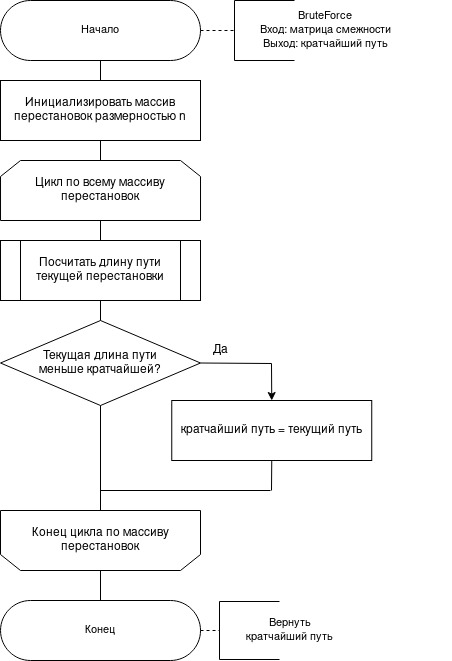
\includegraphics[scale=0.62]{bruteforce.jpg}
		\caption{Схема алгоритма полного перебора.}
		\label{fig:bruteforce}
\end{figure}

\begin{figure}[H]
		\centering
		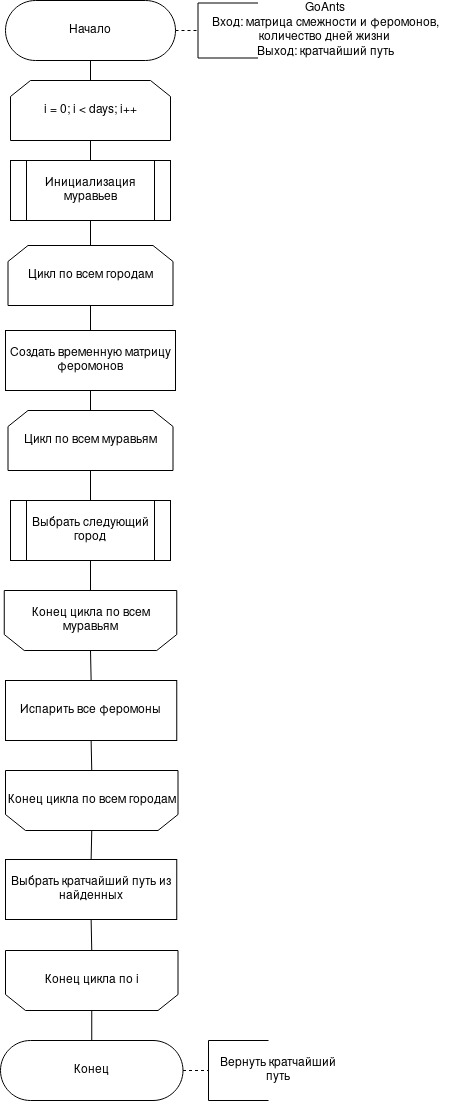
\includegraphics[scale=0.6]{ant.jpg}
		\caption{Схема муравьиного алгоритма.}
		\label{fig:ant}
\end{figure}
	
\section*{Вывод}
	
На основе теоретических данных, полученных аз аналитического раздела, были построенны схемы алгоритмов для решения задачи коммивояжёра.
	
\chapter{Технологическая часть}
	
В данном разделе приведены средства реализации и листинги кода.
	
\section{Требование к ПО}
	
К программе предъявляется ряд требований:
	
\begin{itemize}
	\item на вход подается матрица смежности, со значениями не более чем максимальное целое число деленное пополам;
	\item на выходе -- кратчайший путь.
\end{itemize}
	
\section{Средства реализации}
	
Для реализации ПО был выбран язык программирования С++ \cite{cpp}. Данный язык имеет высокую скорость и
богатую стандартную библиотеку.
	
\section{Реализация алгоритмов}

В листингах 3.1 - 3.2 представлены листинги алгоритмов решения задачи коммивояжёра.
	
\begin{lstlisting}[label=some-code,caption=Алгоритм полного перебора]
double brute::find_shortest_way() {
  std::vector<size_t> route;
  for (size_t i = 0; i < routes.n(); i++)
    route.push_back(i);

  double res = find_route_distance(route);
  while (route_next_step(route)) {
    double cur_res = find_route_distance(route);
    if (cur_res < res)
      res = cur_res;
  }

  return res;
}

double brute::find_route_distance(const std::vector<size_t> &route) {
  double res = 0;
  for (size_t i = 0; i < route.size() - 1; i++) {
    res += routes[route[i]][route[i + 1]];
  }

  res += routes[route[route.size() - 1]][route[0]];

  return res;
}

bool brute::route_next_step(std::vector<size_t> &route) {
  int n = route.size();

  int j = n - 2;
  while (j != -1 && route[j] > route[j + 1])
    j--;

  if (j == -1)
    return false; 

  int k = n - 1;
  while (route[j] > route[k])
    k--;

  std::swap(route[j], route[k]);

  int l = j + 1, r = n - 1; 
  while (l < r)
    std::swap(route[l++], route[r--]);
  return true;
}

\end{lstlisting}
	
\begin{lstlisting}[label=some-code,caption=Муравьиный алгоритм, language=с]
ant_alg::ant_alg(const Matrix<double> &routes, double alpha, double beta,
                 double ro, size_t iterations)
    : routes(routes), alpha(alpha), beta(beta), ro(ro), iterations(iterations) {
  for (size_t i = 0; i < routes.n(); i++) {
    std::vector<double> row_pheromon;
    for (size_t j = i; j < routes.m(); j++)
      row_pheromon.push_back(PHEROMON_START);

    pheromon.push_back(row_pheromon);
  }
}

double ant_alg::find_shortest_way() {
  double res = std::numeric_limits<double>::max();
  for (size_t k = 0; k < iterations; k++) {
    std::vector<std::vector<double>> interests;
    find_interests(interests);

    evaporation();
    for (size_t i = 0; i < routes.n(); i++) {
      ant a(interests, routes.n(), i);
      std::vector<size_t> route = a.get_route();
      double cur_length = route_length(route);
      if (cur_length < res)
        res = cur_length;
      update_pheromon(route, cur_length);
    }
  }

  return res;
}

void ant_alg::update_pheromon(std::vector<size_t> route, double length) {
  double pheromon_step = 1 / length;
  for (size_t i = 0; i < route.size() - 1; i++) {
    if (route[i] < route[i + 1])
      pheromon[route[i]][route[i + 1] - route[i]] += pheromon_step;
    else
      pheromon[route[i + 1]][route[i] - route[i + 1]] += pheromon_step;
  }
  if (route[0] < route[route.size() - 1])
    pheromon[route[0]][route[route.size() - 1] - route[0]] += pheromon_step;
  else
    pheromon[route[route.size() - 1]][route[0] - route[route.size() - 1]] +=
        pheromon_step;
}

double ant_alg::route_length(const std::vector<size_t> &route) {
  double res = 0;
  for (size_t i = 0; i < route.size() - 1; i++) {
    res += routes[route[i]][route[i + 1]];
  }

  res += routes[route[route.size() - 1]][route[0]];

  return res;
}

void ant_alg::evaporation() {
  for (size_t i = 0; i < pheromon.size(); i++)
    for (size_t j = 0; j < pheromon[i].size(); j++) {
      pheromon[i][j] *= (1 - ro);
    }
}

void ant_alg::find_interests(std::vector<std::vector<double>> &intersts) {
  intersts.clear();
  for (size_t i = 0; i < routes.n(); i++) {
    std::vector<double> row_interest;
    for (size_t j = i; j < routes.m(); j++) {
      double interest;
      if (i != j) {
        double t = std::pow(pheromon[i][j - i], alpha);
        double n = std::pow(1 / routes[i][j], beta);
        interest = t * n;

      } else
        interest = 0;
      row_interest.push_back(interest);
    }

    intersts.push_back(row_interest);
  }
}

ant::ant(const std::vector<std::vector<double>> &interests, size_t nodes_count,
         size_t start)
    : interests(interests), nodes_count(nodes_count) {
  route.push_back(start);
}

std::vector<size_t> ant::get_route() {
  find_route();
  return route;
}

void ant::find_route() {
  for (size_t i = 0; i < nodes_count - 1; i++) {
    std::vector<std::pair<size_t, double>> probabilities;
    double interests_sum = 0;
    for (size_t j = 0; j < nodes_count; j++) {
      bool is_visited = false;
      for (size_t k = 0; k < route.size(); k++)
        if (j == route[k])
          is_visited = true;

      if (!is_visited) {
        double interest;
        if (route[i] < j)
          interest = interests[route[i]][j - route[i]];
        else
          interest = interests[j][route[i] - j];

        interests_sum += interest;
        probabilities.push_back(
            std::pair<size_t, double>(j, interest)); // division after loop
      }
    }

    for (size_t j = 0; j < probabilities.size(); j++) {
      probabilities[j].second /= interests_sum;
    }

    double seed = (double)(rand() % 100) / 100.0;
    size_t j = 0;
    double cur_prob = probabilities[0].second;

    while (cur_prob < seed && j + 1 < probabilities.size()) {
      cur_prob += probabilities[++j].second;
    }

    route.push_back(probabilities[j].first);
  }
}

\end{lstlisting}

\section{Тестовые данные}

В таблице \ref{tab:test} приведены тестовые данные. Все тесты были пройденны успешно.

\begin{table}[h!]

	\begin{center}

		\begin{tabular}{c@{\hspace{7mm}}c@{\hspace{7mm}}c@{\hspace{7mm}}c@{\hspace{7mm}}c@{\hspace{7mm}}c@{\hspace{7mm}}}

			\hline

			Матрица смежности & Ожидаемый результат & Полученный результат\\ \hline

			\vspace{4mm}		

			$\begin{bmatrix}

			0 & 3 & 1 & 6 & 8\\

			3 & 0 & 4 & 1 & 0\\

			1 & 4 & 0 & 5 & 0\\

			6 & 1 & 5 & 6 & 1\\

			8 & 0 & 0 & 1 & 0

			\end{bmatrix}$ & 15 & 15\\

			$\begin{bmatrix}

			0 & 10 & 15 & 20\\

			10 & 0 & 35 & 25\\

			15 & 35 & 0 & 30\\

			20 & 25 & 30 & 0

			\end{bmatrix}$ & 80 & 80 \\

			
		\end{tabular}

	\end{center}

	\caption{\label{tab:test} Тестирование алгоритмов.}

\end{table}
	
\section*{Вывод}
	
В данном разделе были разработаны и протестированны алгоритмы решения задачи коммивояжёра.
	
\chapter{Исследовательская часть}
	
В данном разделе приведен анализ характеристик разработанного ПО.

\section{Технические характеристики}
	
Технические характеристики устройства, на котором выполнялось тестирование и исследование, приведены ниже.

\begin{itemize}
	\item Операционная система: Ubuntu Linux 64-bit.
	\item Оперативная память: 16 GB.
	\item Количество логических ядер - 8.
	\item Процессор: Intel(R) Core(TM) i7-8850H CPU @ 2.60GHz \cite{intel}.
\end{itemize}

Тестирование проводилось на компьютере, включенном в сеть электропитания. Во время тестирования компьютер был нагружен только встроенными приложениями окружения рабочего стола, окружением рабочего стола, а также непосредственно системой тестирования. Во время тестирования оптимизации компилятора были отключены.
	
\section{Время выполнения алгоритмов}
	
Время выполнения алгоритм замерялось с помощью многократного вызова функций поиска кратчайшего расстояния и усреденения результата, время перед вызовом функции и после проверялось функцией clock \cite{clock} стандартной библиотеки с++. Количество повторов было подобрано таким образом, чтобы все значения времени выполнения функций были различны, но не занимали избыточно много времени.  Полученные результаты приведены в таблице \ref{tab:timing}.

\begin{table}[H]
	\begin{center}
		\caption{Сравнение времени исполнения алгоритмов решения задачи коммивояжера.}
	    \label{tab:timing}
		\begin{tabular}{|c|c|c|}
			\hline
			\bfseries Размер & \bfseries Муравей & \bfseries Перебор
			\csvreader{inc/time_compare.csv}{}
			{\\\hline \csvcoli&\csvcolii&\csvcoliii}
			\\\hline
		\end{tabular}
	\end{center}
	

\end{table}


\section{Автоматическая параметризация}

В этом разделе расмотрены расхождения результата работы муравьиного алгоритма и эталона при разный классах данных и параметрах муравьиного алгоритма.

\subsection{Класс данных 1}
Расстояния между городами не превосходят 21. Матрица смежности, для которой проводилось тестирование представлена в таблице \ref{tab:mtrv1}

\begin{table}[H]
	\begin{center}
		\begin{tabular}{|1|1|1|1|1|1|1|1|1|1|}
			\hline
			\bfseries & \bfseries & \bfseries & \bfseries & \bfseries & \bfseries & \bfseries & \bfseries & \bfseries & \bfseries
			\csvreader{inc/matrix_20.csv}{}
			{\\\hline \csvcoli&\csvcolii&\csvcoliii&\csvcoliv&\csvcolv&\csvcolvi&\csvcolvii&\csvcolviii&\csvcolix&\csvcolx}
			\\\hline
		\end{tabular}
	\end{center}
	
	\caption{Матрица смежности 1 класса данных.}
	\label{tab:mtrv1}
\end{table}

В таблице \ref{tab:v1} приведена выборка результатов параметризации для матрицы смежности из таблицы \ref{tab:mtrv1}. Количество дней принято равным 20. Полным перебором был посчитан оптимальный путь -- он составил 48.

\begin{table}[H]

	\caption{Выборка из параметризации для матрицы 1 класса данных.}
	\label{tab:v1}
	\begin{center}

		\begin{tabular}{|c@{\hspace{7mm}}|c@{\hspace{7mm}}|c@{\hspace{7mm}}|c@{\hspace{7mm}}|c@{\hspace{7mm}}|c|}

			\hline
			$\alpha$        & $\beta$      & $\rho$      &Длина  & Разница \\

			\hline

0&0&0&64&16\\
0&0&0.4&66&18\\
0&0&0.8&66&18\\
0&0.4&0&59&11\\
0&0.4&0.4&57&9\\
0&0.4&0.8&58&10\\
0&0.8&0&50&2\\
0&0.8&0.4&59&11\\
0&0.8&0.8&52&4\\
\hline
0.4&0&0&66&18\\
0.4&0&0.4&66&18\\
0.4&0&0.8&52&4\\
0.4&0.4&0&61&13\\
0.4&0.4&0.4&58&10\\
0.4&0.4&0.8&60&12\\
0.4&0.8&0&50&2\\
0.4&0.8&0.4&52&4\\
0.4&0.8&0.8&48&0\\
\hline
0.8&0&0&57&9\\
0.8&0&0.4&77&29\\
0.8&0&0.8&61&13\\
0.8&0.4&0&48&0\\
0.8&0.4&0.4&55&7\\
0.8&0.4&0.8&55&7\\
0.8&0.8&0&58&10\\
0.8&0.8&0.4&48&0\\
0.8&0.8&0.8&50&2\\
\hline

		\end{tabular}
	\end{center}
\end{table}

\subsection{Класс данных 2}
Расстояния между городами не превосходят 201. Матрица смежности, для которой проводилось тестирование представлена в таблице \ref{tab:mtrv2}

\begin{table}[H]
	\begin{center}
		\begin{tabular}{|1|1|1|1|1|1|1|1|1|1|}
			\hline
			\bfseries & \bfseries & \bfseries & \bfseries & \bfseries & \bfseries & \bfseries & \bfseries & \bfseries & \bfseries
			\csvreader{inc/matrix_201.csv}{}
			{\\\hline \csvcoli&\csvcolii&\csvcoliii&\csvcoliv&\csvcolv&\csvcolvi&\csvcolvii&\csvcolviii&\csvcolix&\csvcolx}
			\\\hline
		\end{tabular}
	\end{center}
	
	\caption{Матрица смежности 2 класса данных.}
	\label{tab:mtrv2}
\end{table}

В таблице \ref{tab:v2} приведена выборка результатов параметризации для матрицы смежности из таблицы \ref{tab:mtrv2}. Количество дней принято равным 20. Полным перебором был посчитан оптимальный путь -- он составил 421.

\begin{table}[H]

	\caption{Выборка из параметризации для матрицы 2 класса данных.}
	\label{tab:v2}
	\begin{center}

		\begin{tabular}{|c@{\hspace{7mm}}|c@{\hspace{7mm}}|c@{\hspace{7mm}}|c@{\hspace{7mm}}|c@{\hspace{7mm}}|c|}

			\hline
			$\alpha$        & $\beta$      & $\rho$      &Длина  & Разница \\

			\hline

0&0&0&707&286\\
0&0&0.4&595&174\\
0&0&0.8&604&183\\
0&0.4&0&562&141\\
0&0.4&0.4&511&90\\
0&0.4&0.8&624&203\\
0&0.8&0&493&72\\
0&0.8&0.4&421&0\\
0&0.8&0.8&511&90\\
\hline
0.4&0&0&687&266\\
0.4&0&0.4&583&162\\
0.4&0&0.8&593&172\\
0.4&0.4&0&595&174\\
0.4&0.4&0.4&631&210\\
0.4&0.4&0.8&518&97\\
0.4&0.8&0&493&72\\
0.4&0.8&0.4&421&0\\
0.4&0.8&0.8&477&56\\
\hline
0.8&0&0&646&225\\
0.8&0&0.4&685&264\\
0.8&0&0.8&712&291\\
0.8&0.4&0&514&93\\
0.8&0.4&0.4&493&72\\
0.8&0.4&0.8&421&0\\
0.8&0.8&0&493&72\\
0.8&0.8&0.4&421&0\\
0.8&0.8&0.8&421&0\\
\hline

		\end{tabular}
	\end{center}
\end{table}

\subsection{Класс данных 3}
Расстояния между городами не превосходят 2001. Матрица смежности, для которой проводилось тестирование представлена в таблице \ref{tab:mtrv3}

\begin{table}[H]
	\begin{center}
		\begin{tabular}{|1|1|1|1|1|1|1|1|1|1|}
			\hline
			\bfseries & \bfseries & \bfseries & \bfseries & \bfseries & \bfseries & \bfseries & \bfseries & \bfseries & \bfseries
			\csvreader{inc/matrix_2001.csv}{}
			{\\\hline \csvcoli&\csvcolii&\csvcoliii&\csvcoliv&\csvcolv&\csvcolvi&\csvcolvii&\csvcolviii&\csvcolix&\csvcolx}
			\\\hline
		\end{tabular}
	\end{center}
	
	\caption{Матрица смежности 3 класса данных.}
	\label{tab:mtrv3}
\end{table}

В таблице \ref{tab:v3} приведена выборка результатов параметризации для матрицы смежности из таблицы \ref{tab:mtrv3}. Количество дней принято равным 20. Полным перебором был посчитан оптимальный путь -- он составил 4503.

\begin{table}[H]

	\caption{Выборка из параметризации для матрицы 3 класса данных.}
	\label{tab:v3}
	\begin{center}

		\begin{tabular}{|c@{\hspace{7mm}}|c@{\hspace{7mm}}|c@{\hspace{7mm}}|c@{\hspace{7mm}}|c@{\hspace{7mm}}|c|}

			\hline
			$\alpha$        & $\beta$      & $\rho$      &Длина  & Разница \\

			\hline

0&0&0&5533&1030\\
0&0&0.4&6525&2022\\
0&0&0.8&6407&1904\\
0&0.4&0&5656&1153\\
0&0.4&0.4&4583&80\\
0&0.4&0.8&5174&671\\
0&0.8&0&4503&0\\
0&0.8&0.4&4903&400\\
0&0.8&0.8&4712&209\\
\hline
0.4&0&0&6258&1755\\
0.4&0&0.4&6267&1764\\
0.4&0&0.8&6225&1722\\
0.4&0.4&0&5705&1202\\
0.4&0.4&0.4&4821&318\\
0.4&0.4&0.8&4712&209\\
0.4&0.8&0&5024&521\\
0.4&0.8&0.4&4712&209\\
0.4&0.8&0.8&4820&317\\
\hline
0.8&0&0&5878&1375\\
0.8&0&0.4&5785&1282\\
0.8&0&0.8&6586&2083\\
0.8&0.4&0&5074&571\\
0.8&0.4&0.4&4893&390\\
0.8&0.4&0.8&4503&0\\
0.8&0.8&0&4857&354\\
0.8&0.8&0.4&4503&0\\
0.8&0.8&0.8&4712&209\\
\hline

		\end{tabular}
	\end{center}
\end{table}

\section*{Вывод}

При небольших размерах графа (от 3 до 6) алгоритм полного перебора выигрывает по времени у муравьиного. Например, при размере графа 6, полный перебор работает быстрее примерно в 10 раз. Однако, при увеличении размера графа (от 7 и выше), ситуация меняется в обратную сторону: муравьиный алгоритм начинает значительно выигрывать по времени у алгоритма полного перебора. При размере графа = 10, муравьиный алгоритм работает в 400 раз быстрее.

Наиболее стабильные результаты автоматической параметризации получаются при наборе $\alpha = 0.4$, $\beta = 0.8$, $\rho = $ любое. При таких параметрах полученный результат не отличается более чем на 1 от эталонного, и, в около 75\% (на промежутке $\rho = 0.0..1.0$) случаев полученный результат совпадает с эталонным. Наиболее нестабильные результаты полученны при $\alpha = 1.0$, $\beta = 0.0$, $\rho = $ любое.

\chapter*{Заключение}
\addcontentsline{toc}{chapter}{Заключение}
	
В рамках данной лабораторной работы лабораторной работы была достигнута её цель: изучен муравьиный алгоритм и приобретены навыки параметризации методов на примере муравьиного алгоритма. Также выполнены следующие задачи:
	
\begin{itemize}
	\item реализованны два алгоритма решения задачи коммивояжера;
	\item замерено время выполнения алгоритмов;
	\item муравьиный алгоритм протестирован на разных переменных;
	\item сделаны выводы на основе проделанной работы;
\end{itemize}

Использовать муравьиный алгоритм для решения задачи коммивояжера выгодно (с точки зрения времени выполнения), в сравнении с алгоритмом полного перебора, в случае если в анализируемом графе вершин больше либо равно 9. Так, например, при размере графа 11, муравьиный алгоритм работает быстрее чем алгоритм полного перебора в 15 раз. Стоит отметить, что муравьиный алгоритм не гарантирует что найденный путь будем оптимальным, так как он является эвристическим алгоритмом, в отличии от алгоритма полного перебора.

\addcontentsline{toc}{chapter}{Литература}
\bibliographystyle{utf8gost705u}  % стилевой файл для оформления по ГОСТу
\bibliography{51-biblio}          % имя библиографической базы (bib-файла)
	
\end{document}
